
\begin{figure}
  \def\frac{0.32}
    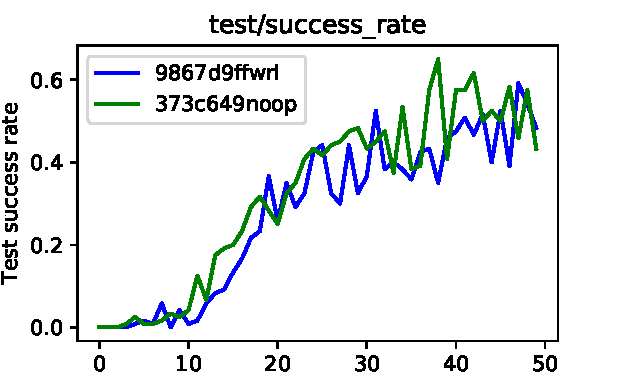
\includegraphics[width=\frac\columnwidth]{media/res/373c649_FetchSlide-v1-noop/test/success_rate.pdf}%
    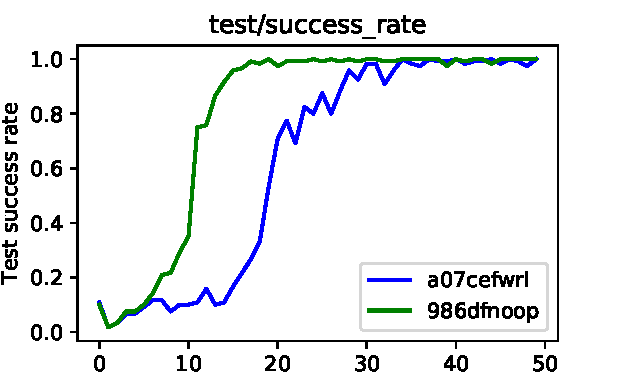
\includegraphics[width=\frac\columnwidth]{media/res/a077c9e_FetchPush-v1-fwrl/test/success_rate.pdf}%
    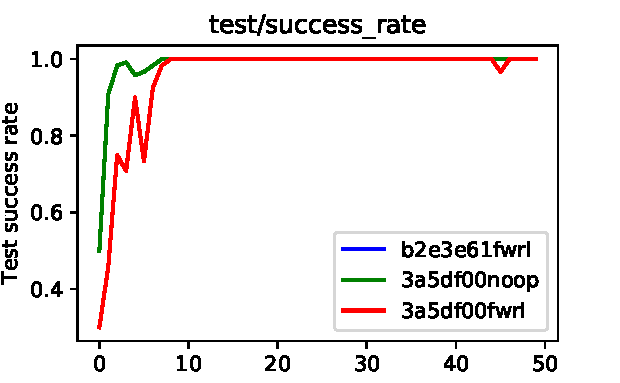
\includegraphics[width=\frac\columnwidth]{media/res/3a5df00_FetchReach-v1-fwrl/test/success_rate.pdf}\\
    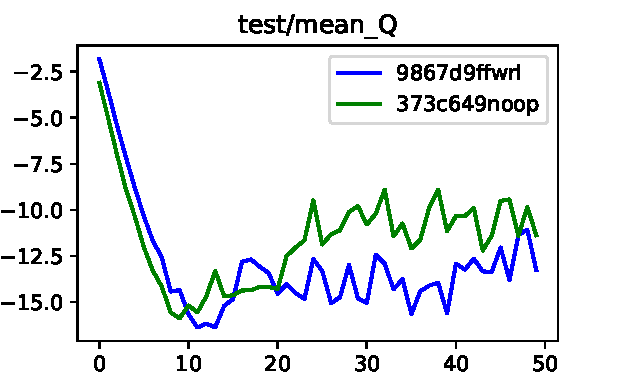
\includegraphics[width=\frac\columnwidth]{media/res/373c649_FetchSlide-v1-noop/test/mean_Q.pdf}%
    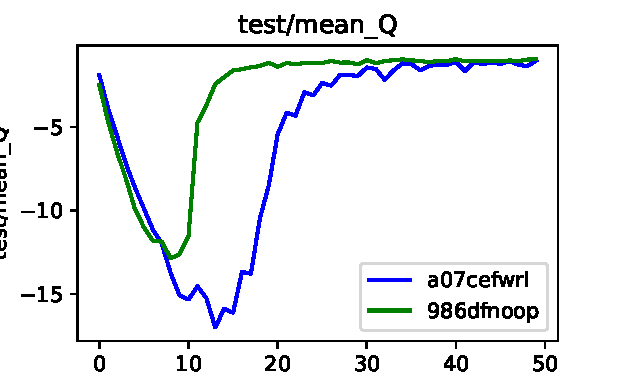
\includegraphics[width=\frac\columnwidth]{media/res/a077c9e_FetchPush-v1-fwrl/test/mean_Q.pdf}%
    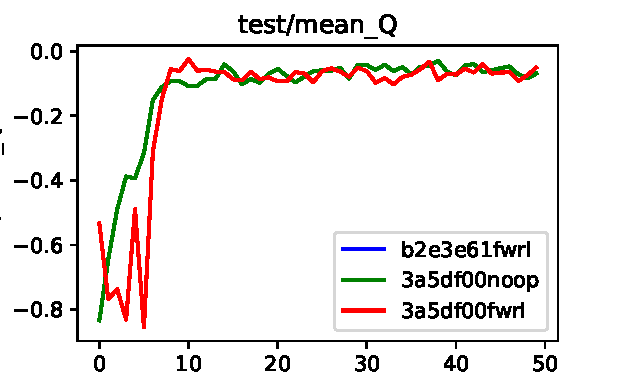
\includegraphics[width=\frac\columnwidth]{media/res/3a5df00_FetchReach-v1-fwrl/test/mean_Q.pdf}
    \caption{fwrl = Floyd Warshall (lower bound only) + HER; noop = HER.
  Test success rate and Mean Q on (1) Fetch-Slide, (2) Fetch-Push and (3)
  Fetch-Reach task}
    \label{fig:fetch-slide-success}
\end{figure}


%
\begin{figure}%
  \def\frac{0.24}
  With HER sampling:\\
  \includegraphics[width=\frac\columnwidth]{media/res/3a90344-FetchReach-v1-stepfwrl-future/test/success_rate.pdf}%
  \includegraphics[width=\frac\columnwidth]{media/res/3a90344-FetchReach-v1-stepfwrl-future/test/mean_Q.pdf}%
  \includegraphics[width=\frac\columnwidth]{media/res/3a90344-FetchReach-v1-stepfwrl-future/train/critic_loss.pdf}%
  \includegraphics[width=\frac\columnwidth]{media/res/3a90344-FetchReach-v1-stepfwrl-future/train/critic_addnl_loss.pdf}\\
  Without HER sampling:\\
  \includegraphics[width=\frac\columnwidth]{media/res/d047a03-FetchReach-v1-stepfwrl-none/test/success_rate.pdf}%
  \includegraphics[width=\frac\columnwidth]{media/res/d047a03-FetchReach-v1-stepfwrl-none/test/mean_Q.pdf}%
  \includegraphics[width=\frac\columnwidth]{media/res/d047a03-FetchReach-v1-stepfwrl-none/train/critic_loss.pdf}%
  \includegraphics[width=\frac\columnwidth]{media/res/d047a03-FetchReach-v1-stepfwrl-none/train/critic_addnl_loss.pdf}\\
Using both upper and lower bound in FWRL\\
  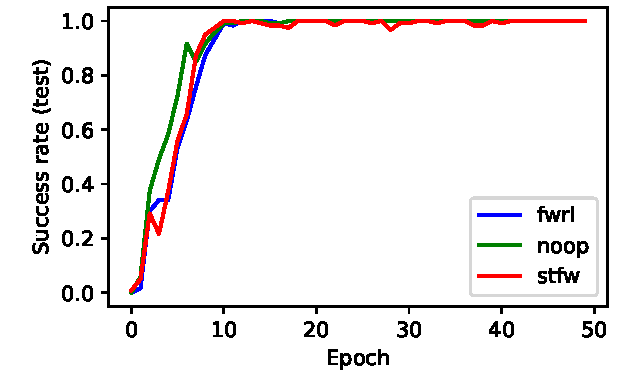
\includegraphics[width=\frac\columnwidth]{media/res/f0d4cfa-FetchReach-v1-stfw-none/test/success_rate.pdf}%
  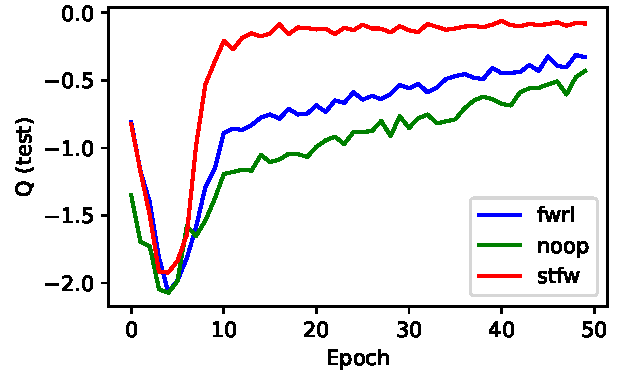
\includegraphics[width=\frac\columnwidth]{media/res/f0d4cfa-FetchReach-v1-stfw-none/test/mean_Q.pdf}%
  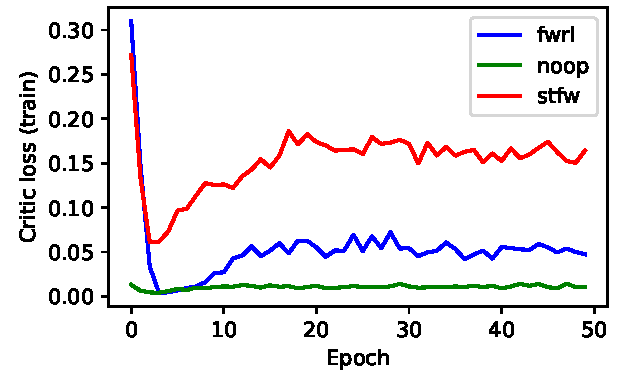
\includegraphics[width=\frac\columnwidth]{media/res/f0d4cfa-FetchReach-v1-stfw-none/train/critic_loss.pdf}%
  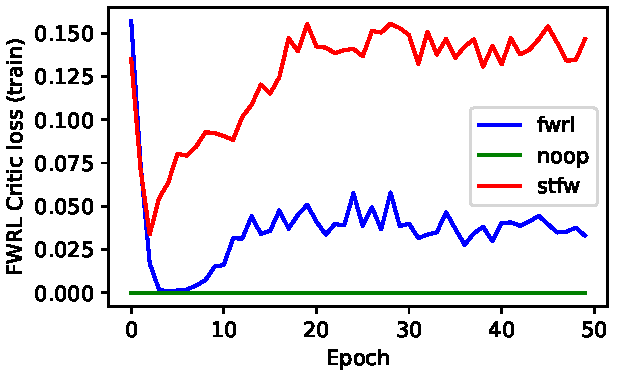
\includegraphics[width=\frac\columnwidth]{media/res/f0d4cfa-FetchReach-v1-stfw-none/train/critic_addnl_loss.pdf}\\
  \caption{
    stepfwrl = DDPG loss + Step loss + FWRL constraints, noop = DDPG loss + HER
    sampling, fwrl = DDPG Loss + FWRL constraints.
    All experiments on Fetch-Reach task.
  }%
  \label{fig:fwrl-stepfwrl-noop-FetchReach}%
\end{figure}%
% 

%
\begin{figure}%
  \def\frac{0.24}
  With HER sampling\\
  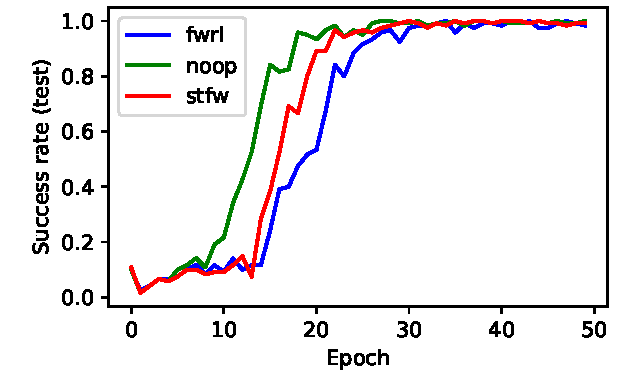
\includegraphics[width=\frac\columnwidth]{media/res/ea0e35b-FetchPush-v1-stfw-future/test/success_rate.pdf}%
  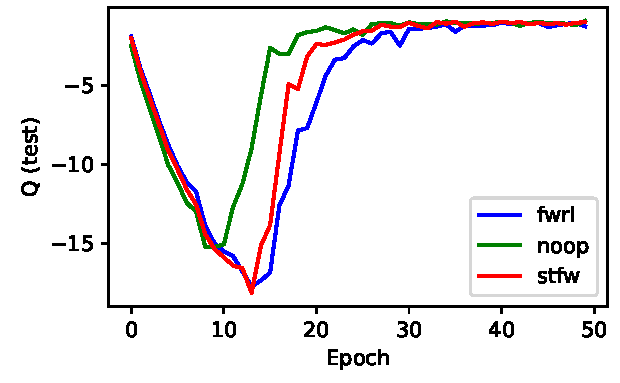
\includegraphics[width=\frac\columnwidth]{media/res/ea0e35b-FetchPush-v1-stfw-future/test/mean_Q.pdf}%
  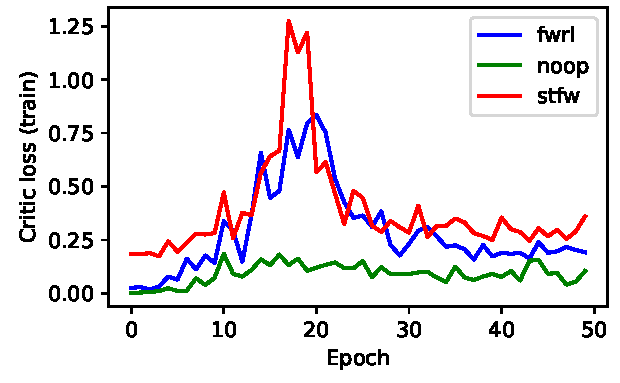
\includegraphics[width=\frac\columnwidth]{media/res/ea0e35b-FetchPush-v1-stfw-future/train/critic_loss.pdf}%
  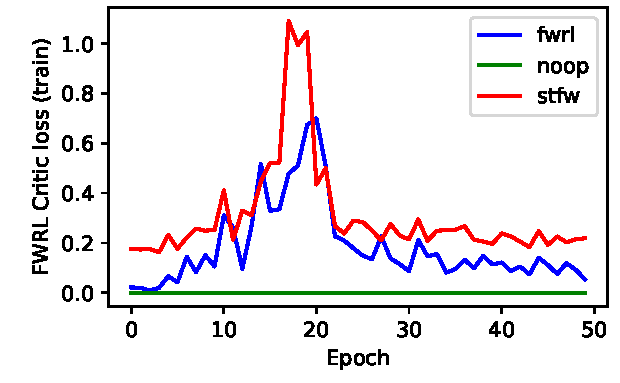
\includegraphics[width=\frac\columnwidth]{media/res/ea0e35b-FetchPush-v1-stfw-future/train/critic_addnl_loss.pdf}\\
  Without HER sampling\\
  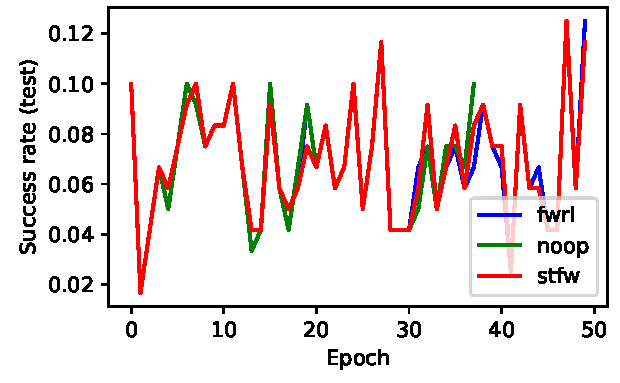
\includegraphics[width=\frac\columnwidth]{media/res/ea0e35b-FetchPush-v1-stfw-none/test/success_rate.pdf}%
  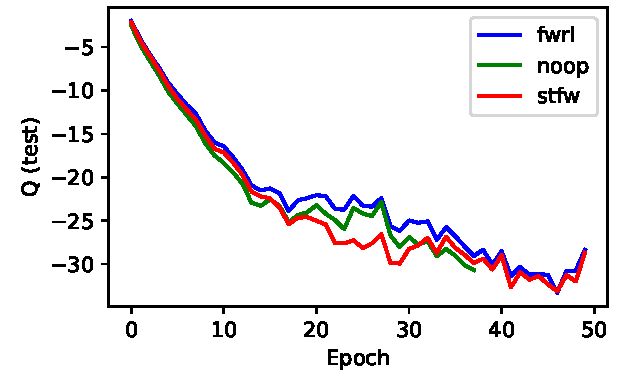
\includegraphics[width=\frac\columnwidth]{media/res/ea0e35b-FetchPush-v1-stfw-none/test/mean_Q.pdf}%
  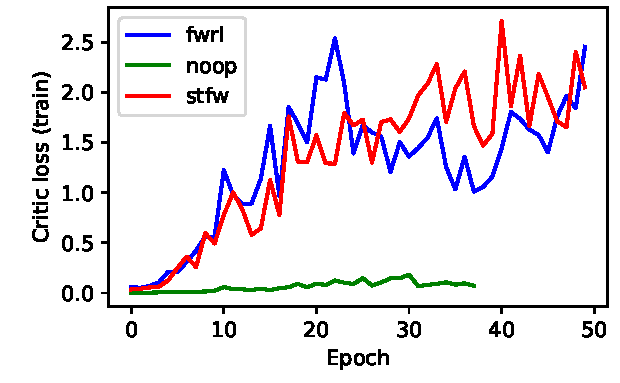
\includegraphics[width=\frac\columnwidth]{media/res/ea0e35b-FetchPush-v1-stfw-none/train/critic_loss.pdf}%
  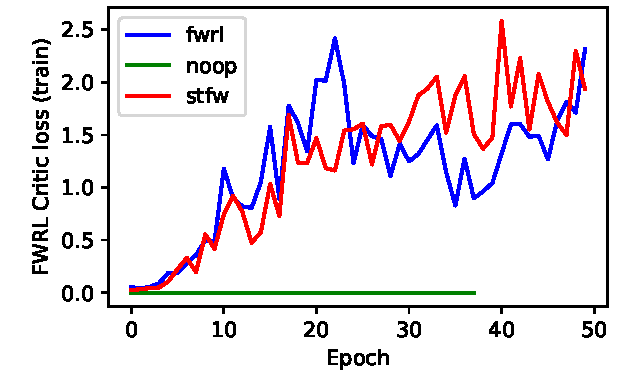
\includegraphics[width=\frac\columnwidth]{media/res/ea0e35b-FetchPush-v1-stfw-none/train/critic_addnl_loss.pdf}%
  \caption{noop = DDPG loss, fwrl = DDPG + FWRL bounds,
    stfw = DDPG loss + Step loss + FWRL bounds. All experiments on Fetch-Push}
  \label{fig:loss-func-fetch-push}
\end{figure}
%